\chapter{システムの実装}
\label{chap:poordirection}

\section{車両認識システム}
本研究にて構築するシステムは, 主に「iOSアプリケーション」, 「Webアプリケーション」, 「データベース」の三要素にて成り立つ(図3.1).

\subsection{システムの流れ}
本研究にて構築するシステムは,
\begin{screen}
\begin{itembox}[l]{iOSアプリケーション}
\begin{enumerate}
\item iOSアプリケーションにて車両のナンバープレートを撮影する.
\item iOSアプリケーションの内部処理にて, 撮影画像から車両ナンバーを文字列として取得する.
\item 取得した車両ナンバーをWebアプリケーション側のPostgreSQLに送信する.
\end{enumerate}
\end{itembox}

\begin{itembox}[l]{Webアプリケーション}
\begin{enumerate}
\item Webアプリケーションにログインする.
\item PostgreSQLデータベースに各種操作を行う.
\item Webアプリケーションからログアウトする.
\end{enumerate}
\end{itembox}
\end{screen}
という流れを想定して開発した.

\begin{figure}
\begin{center}
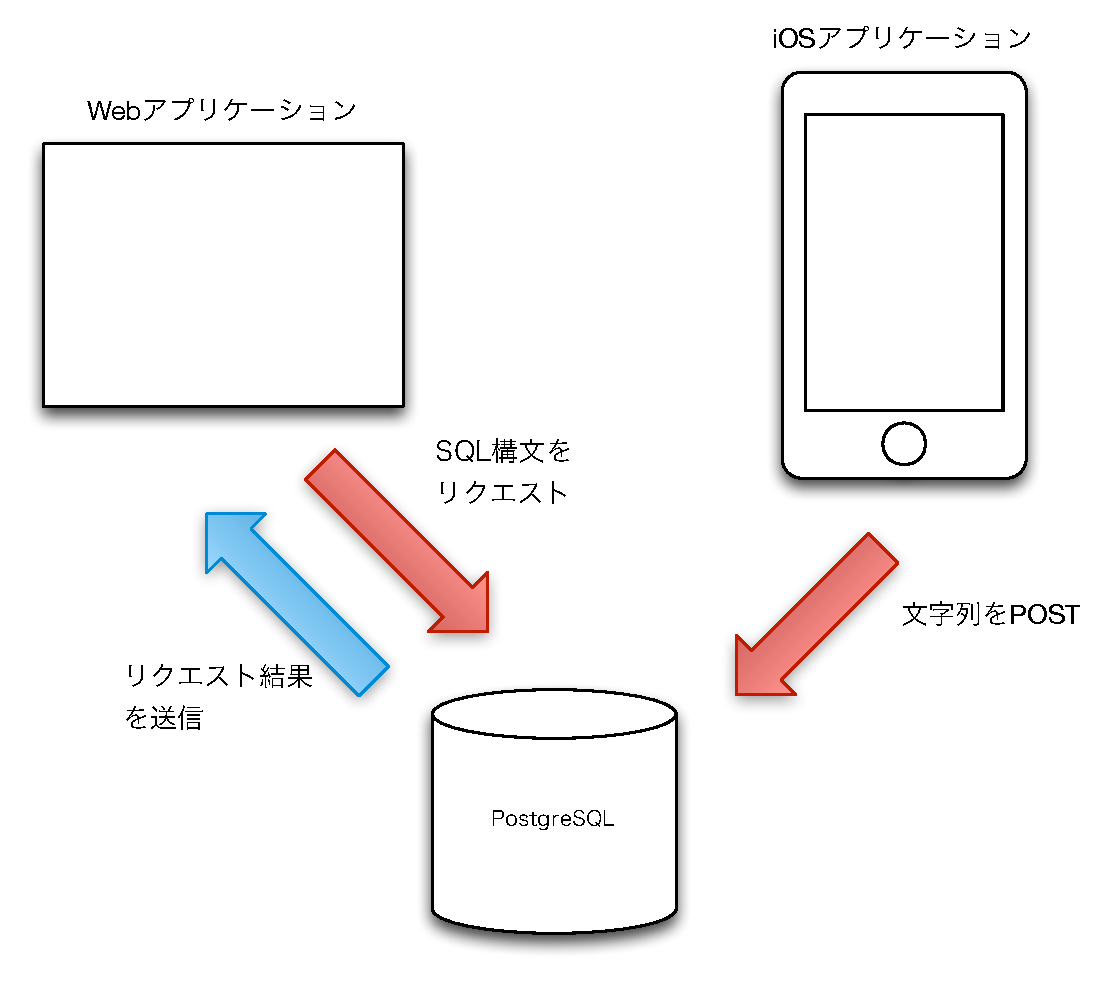
\includegraphics[width=16cm]{fig/system.pdf}
\end{center}
\caption{車両ナンバー認識システムの簡易システム図}
\end{figure}

\begin{figure}
\begin{center}
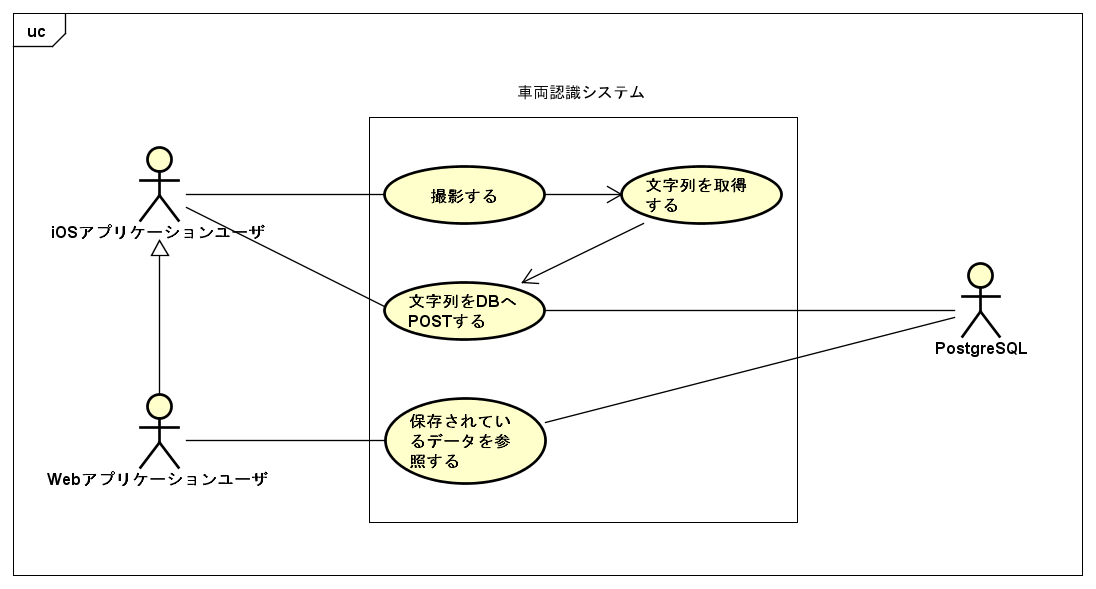
\includegraphics[width=16cm]{fig/usecase_system.png}
\end{center}
\caption{車両ナンバー認識システムのユースケース図}
\end{figure}

\section{iOSアプリケーション}
iOSアプリケーションを作成するにあたり, 以下の言語とライブラリ, 統合開発環境を利用した(表3.1).

\begin{table}
\begin{center}
\begin{tabular}{|l|l|} \hline
Xcode &  \\ \hline
Objective-C 2.0 & \\ \hline
Tesseract-OCR & \\ \hline
OpenCV & \\ \hline
\end{tabular}
\end{center}
\caption{iOSアプリケーション作成時に利用した環境のバージョン一覧}
\end{table}

\subsection{要件定義}
iOSアプリケーションには, 以下の機能を実装する.
\begin{screen}
\begin{itemize}
\item iOSデバイスのカメラにて撮影する
\item 撮影画像から目的の文字列を取得する
\item 取得した文字列をWebアプリケーションのデータベースにPOSTする.
\end{itemize}
\end{screen}

これらの要件を, UMLを用いて分析する.

\subsection{ユースケース}
ユーザがiOSデバイスのカメラを用いて撮影した画像から, 文字列を検出する.
その文字列をWebアプリケーションのデータベースに送信し, 集積する(図3.3).

\begin{figure}
\begin{center}
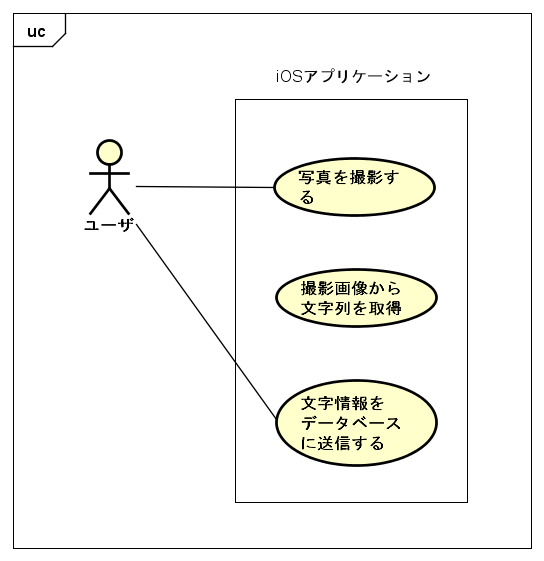
\includegraphics[width=16cm]{fig/usecase_ios.png}
\end{center}
\caption{iOSアプリケーションのユースケース図}
\end{figure}

\subsection{クラス}
\begin{figure}
\begin{center}
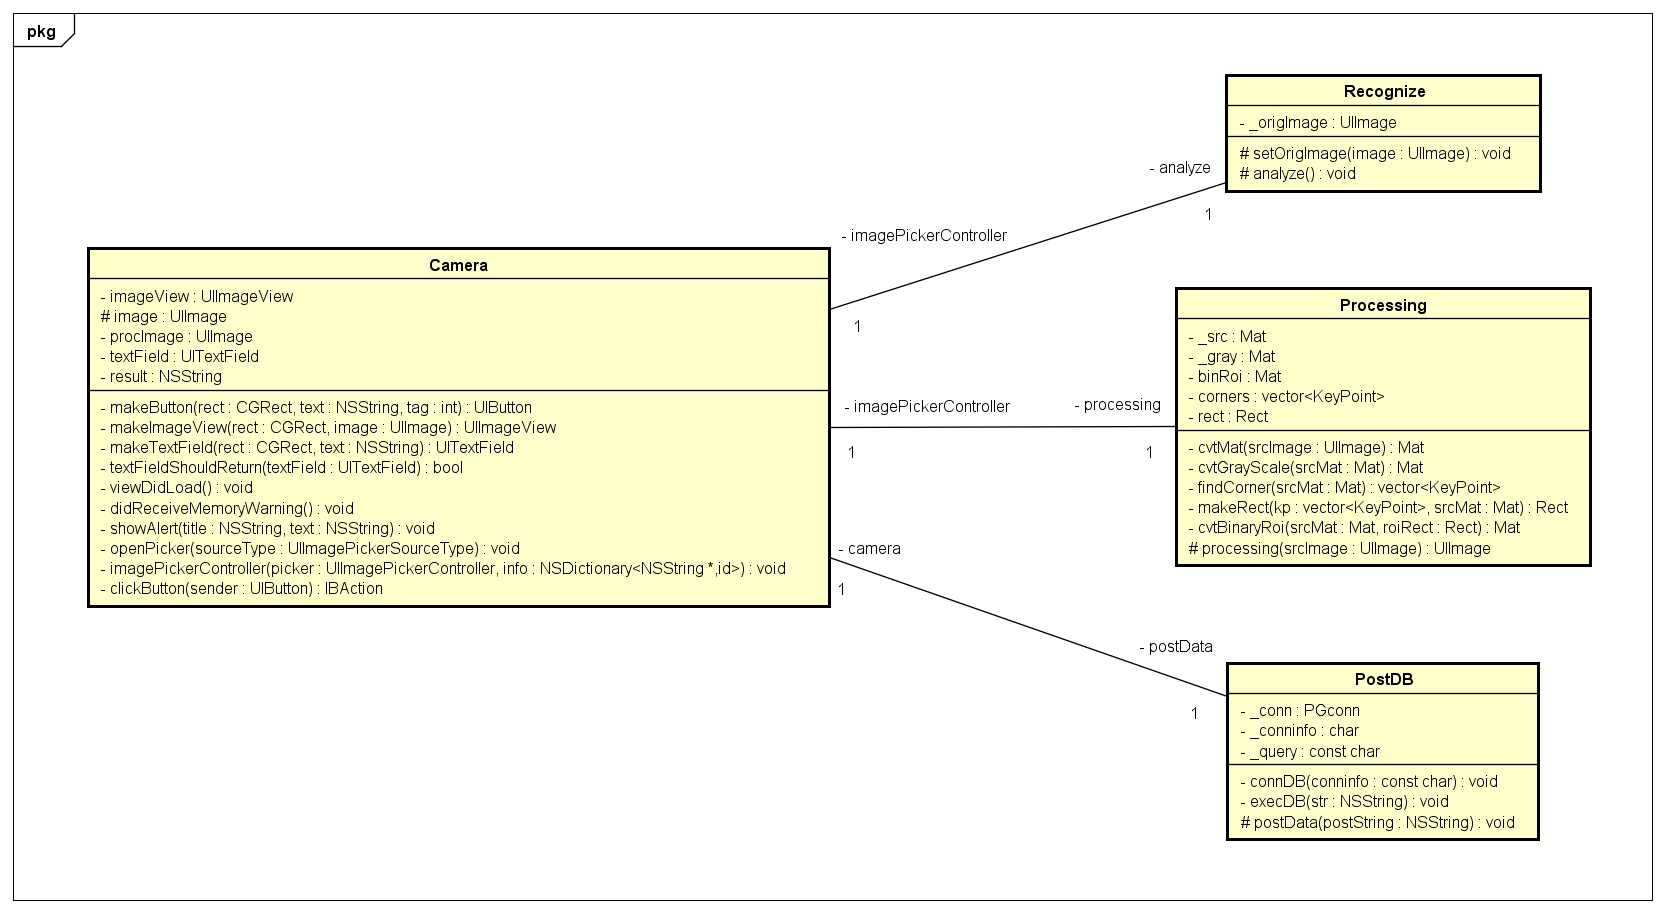
\includegraphics[width=16cm]{fig/class_ios.png}
\end{center}
\caption{iOSアプリケーションのクラス図}
\end{figure}

\begin{description}

\item (A) Cameraクラス

Cameraクラスでは, 「iOSアプリケーションのMainViewにボタン等を配置する」, 「iOSデバイスのカメラを起動し, 撮影した画像を保存する」, 「他クラスのメソッドを呼び出す」ことが可能である.

\begin{itemize}
\item 属性

\begin{breakbox}
\begin{itemize}
\item imageView:UIImageView

撮影した画像を出力するためのローカル変数.

\item image:UIImage

撮影した画像.

\item procImage:UIImage

Processingクラスにて画像処理された画像.

\item textField:UITextField

Recognizeクラスにて取得した文字列を表示するためのテキストボックス.

\item result:NSString

Recognizeクラスにて取得してきた文字列.
\end{itemize}
\end{breakbox}

\item 操作

\begin{itembox}[l]{makeButton:UIButton}
iOSアプリケーションのMainViewにボタンを作成するメソッド.

ボタンを配置する座標, サイズ, ボタンに書かれる文字列, ボタンに付加するタグを指定して呼び出すことで, iOSアプリケーションのMainViewにボタンを作成し配置する.

\begin{itembox}[l]{引数}
\begin{itemize}
\item rect:CGRect

ボタンの座標, サイズを決定する変数.

\item text:NSString

ボタンに書かれる文字列を決定する変数.

\item tag:int

ボタンに整数型のタグを付加するための変数.
\end{itemize}
\end{itembox}
\end{itembox}

\begin{itembox}[l]{makeImage:UIImageView}
iOSアプリケーションのMainViewに画像を表示するためのSubViewを作成するメソッド.

画像を配置する座標, サイズ, 出力する画像を指定して呼び出すことで, iOSアプリケーションのMainViewに画像を出力する.

\begin{itembox}[l]{引数}
\begin{itemize}
\item rect:CGRect

画像を出力するSubViewの座標, サイズを指定する変数.

\item image:UIImage

SubViewに出力する画像を指定する変数.
\end{itemize}
\end{itembox}
\end{itembox}

\begin{itembox}[l]{makeTextField:UITextField}
iOSアプリケーションのMainViewにテキストフィールドを作成するメソッド.

テキストフィールドを配置する座標, サイズ, 入力されるテキストを指定して呼び出すことで, iOSアプリケーションのMainViewにテキストフィールドを作成し配置する.

\begin{itembox}[l]{引数}
\begin{itemize}
\item rect:CGRect

テキストフィールドを配置する座標, サイズを指定する変数.

\item text:NSString

テキストフィールドに入力する文字列を指定する変数.
\end{itemize}
\end{itembox}
\end{itembox}

\begin{itembox}[l]{textFieldShouldReturn:BOOL}
テキストフィールドにて, キーボードでリターンキーを押した際の挙動を制御するメソッド.

文字列を編集後にリターンキーを押した際に呼び出され, SubViewとして呼びだされているキーボードを引っ込める.

\begin{itembox}[l]{引数}
\begin{itemize}
\item textField:UITextField

編集したい文字列が入力されているテキストフィールド.
\end{itemize}
\end{itembox}
\end{itembox}

\begin{itembox}[l]{viewDidLoad:void}
アプリケーションが起動した際に一度だけ読み込まれるメソッド.

変数の初期化やMainViewにボタン等を配置する際に利用する.
\end{itembox}

\begin{itembox}[l]{didReceiveMemoryWarning:void}
iOSアプリケーション使用時に, メモリが不足する際に呼び出されるメソッド.

すべてのViewに対して参照を開放する際に利用する.
\end{itembox}

\begin{itembox}[l]{showAlert:void}
アラートビューを表示するメソッド.

アラートビューのタイトルと表示するアラートの内容を指定して呼び出すことで, iOSアプリケーションのMainView上にSubViewとしてアラートが表示される.

\begin{itembox}[l]{引数}
\begin{itemize}
\item title:NSString

アラートビューのタイトルを指定する変数.

\item text:NSString

アラートビューに表示するテキストを指定する変数.
\end{itemize}
\end{itembox}
\end{itembox}

\begin{itembox}[l]{openPicker:void}
iOSアプリケーションにて, 画像を取得するためのメソッド.

カメラ, フォトアルバム, フォトライブラリから画像を取得する.

このメソッドでは, iOSのカメラ機能にて撮影した画像を取得する際に呼び出す.

\begin{itembox}[l]{引数}
\begin{itemize}
\item sourceType:UIImagePickerSourceType

イメージピッカーの属性を決定する変数.
カメラ, フォトアルバム, フォトライブラリのいずれかから選択する.
\end{itemize}
\end{itembox}
\end{itembox}

\begin{itembox}[l]{imagePickercontroller:void}
画像取得後に呼び出されるメソッド.

画像を取得した後の処理を行う他クラスのメソッドを呼び出す.

\begin{itembox}[l]{引数}
\begin{itemize}
\item picker:UIImagePickerController

画像取得元のイメージピッカーを指定する変数.

\item info:NSDictionary$<$NSString *, id$>$

取得した画像の情報を格納する変数.
\end{itemize}
\end{itembox}
\end{itembox}

\begin{itembox}[l]{clickButton:IBAction}
iOSアプリケーション上のMainViewに配置されているボタンを押下した際に呼び出されるメソッド.

\begin{itembox}[l]{引数}
\begin{itemize}
\item sender:UIButton

どのボタンが押下されたのかを決定する変数.
\end{itemize}
\end{itembox}
\end{itembox}

\end{itemize}


\item (B) Processingクラス

Processingクラスでは, 「撮影画像をOpenCVにて加工可能となるように処理を施す」, 「撮影画像中の文字列が含まれている箇所に注目する」, 「注目している箇所のみで光学的文字認識が施されるように, 撮影画像を加工する」ことが可能である.

\begin{itemize}
\item 属性

\begin{breakbox}
\begin{itemize}
\item \_src:Mat

入力画像を指定する変数.

\item \_gray:Mat

グレースケール変換された画像を格納する変数.

\item binRoi:Mat

バイナリスケール変換された画像を格納する変数.

\item corners:vector$<$KeyPoint$>$

検出した特徴点を格納する変数.

\item rect:Rect

特徴点を内包した矩形の座標, サイズ決定する変数.

\end{itemize}
\end{breakbox}

\newpage

\item 操作

\begin{itembox}[l]{cvtMat:Mat}
UIImage型の画像をMat型に変換するメソッド.

UIImage型の入力画像を指定して呼び出すことで, OpenCVで処理可能なMat型に変換する.

\begin{itembox}[l]{srcImage:UIImage}
\begin{itemize}
\item srcImage:UIImage

UIImage型の画像を格納する変数.
\end{itemize}
\end{itembox}
\end{itembox}

\begin{itembox}[l]{cvtGrayMat:Mat}
Mat型画像をグレースケール化するメソッド.

cvtMatにてMat型に変換した入力画像にグレースケール化処理を施す.

\begin{itembox}[l]{引数}
\begin{itemize}
\item srcMat:Mat

3チャネルの入力カラー画像を格納する変数.
\end{itemize}
\end{itembox}
\end{itembox}

\begin{itembox}[l]{findCorner:vector$<$KeyPoint$>$}
グレースケール画像から特徴点を検出するメソッド.

cvtGrayScaleにてグレースケール処理を施した画像を指定することで, その画像中から特徴点を検出する.

\begin{itembox}[l]{引数}
\begin{itemize}
\item srcMat:Mat

グレースケール画像を格納する変数.
\end{itemize}
\end{itembox}
\end{itembox}

\begin{itembox}[l]{makeRect:Rect}
特徴点を内包する矩形の座標, サイズを決定するメソッド.

特徴点の集合を指定することで, 特徴点の多い部分に注目するための矩形を設定する.

\begin{itembox}[l]{引数}
\begin{itemize}
\item kp:vector$<$KeyPoint$>$

特徴点の集合を格納する変数.

\item srcMat:Mat

グレースケール画像を格納するための変数.
\end{itemize}
\end{itembox}
\end{itembox}

\begin{itembox}[l]{cvyBinaryRoi:Mat}
Mat型カラー画像をバイナリ画像へ変換するメソッド.

makeRectにて設定した矩形を指定することで, 注目している範囲をバイナリ画像化する.

\begin{itembox}[l]{引数}
\begin{itemize}
\item srcMat:Mat

3チャネルの入力カラー画像を格納する変数.

\item roiRect:Rect

注目する矩形範囲を決定する変数.
\end{itemize}
\end{itembox}
\end{itembox}

\begin{itembox}[l]{provessing:UIImage}
Processingクラスのメソッドをコントロールするメソッド.

\begin{itembox}[l]{引数}
\begin{itemize}
\item srcImage:UIImage

CameraクラスのopenPickerControllerメソッドにて取得した撮影画像を格納する変数.
\end{itemize}
\end{itembox}
\end{itembox}
\end{itemize}

\newpage

\item (C) Recognizeクラス

Recognizeクラスでは, 「光学的文字認識を実行する」, 「取得した文字列をCameraクラスに渡す」ことが可能である.

\begin{itemize}
\item 属性

\begin{breakbox}
\begin{itemize}
\item \_origImage:UIImage

光学的文字認識を実行する画像を格納するための変数.
\end{itemize}
\end{breakbox}

\item 操作

\begin{itembox}[l]{setOrigImage:void}
光学的文字認識を実行する画像を取得するためのメソッド.

Processingクラスのprocessingメソッドにて処理の施された画像を受け取り, \_origImageに格納する.

\begin{itembox}[l]{引数}
\begin{itemize}
\item image:UIImage

光学的文字認識を施す画像を指定する変数.
\end{itemize}
\end{itembox}
\end{itembox}

\begin{itembox}[l]{analyze:void}
Tesseract-OCRによる光学的文字認識を実行するメソッド.
\end{itembox}
\end{itemize}

\item (D) PostDBクラス
\begin{itemize}
\item 属性

\begin{breakbox}
\begin{itemize}
\item \_conn:PGconn

PostgreSQLデータベースとの接続状態を格納する構造体.

\item \_conninfo:const char

PostgreSQLデータベースの接続する際に必要となる情報を格納する変数.

\item \_query:char

接続したPostgreSQLにて実行するクエリを決定する変数.
\end{itemize}
\end{breakbox}

\item 操作

\begin{itembox}[l]{connDB:void}
WebアプリケーションのPostgreSQLに接続するメソッド.

\begin{itembox}[l]{引数}
\begin{itemize}
\item conninfo:const char

PostgreSQLへの接続状態を保存する変数.
\end{itemize}
\end{itembox}
\end{itembox}

\begin{itembox}[l]{execDB:void}
WebアプリケーションのPostgreSQLデータベースへクエリを発行し, データベースへデータを追加する.

\begin{itembox}[l]{引数}
\begin{itemize}
\item str:NSString

PostgreSQLデータベースへ送信する文字列を決定する変数.
\end{itemize}
\end{itembox}
\end{itembox}

\begin{itembox}[l]{postData:void}
PostDBクラスのメソッドをコントロールするメソッド.

\begin{itembox}[l]{引数}
\begin{itemize}
\item postString:NSString

WebアプリケーションのPostgreSQLデータベースへ送信する文字列を決定する変数.
\end{itemize}
\end{itembox}
\end{itembox}

\end{itemize}

\end{description}

\section{Webアプリケーション}
Webアプリケーションを作成するにあたり, 以下の言語とライブラリ, サービスを利用した(表3.2).

\begin{table}
\begin{center}
\begin{tabular}{|l|l|} \hline
rbenv & \\ \hline
Ruby & \\ \hline
RubyGems & \\ \hline
Ruby on Rails & \\ \hline
PostgreSQL & \\ \hline
Heroku & \\ \hline
\end{tabular}
\end{center}
\caption{Webアプリケーション作成時に利用した環境のバージョン一覧}
\end{table}

\subsection{要件定義}
Webアプリケーションには, 以下の機能を実装する.

\begin{screen}
\begin{itemize}
\item データベースにて, iOSアプリケーションから送信された文字列を送信された日時/時刻とともに管理する.

\item 集積したデータを文字列, 日付にて検索する.
\end{itemize}
\end{screen}

これらの要件を, UMLを用いて分析する.

\subsection{ユースケース}
ユーザはiOSアプリケーションから送信された全データを閲覧することができ, 文字列, 送信した日付で検索することができる(図3.5).

\begin{figure}
\begin{center}
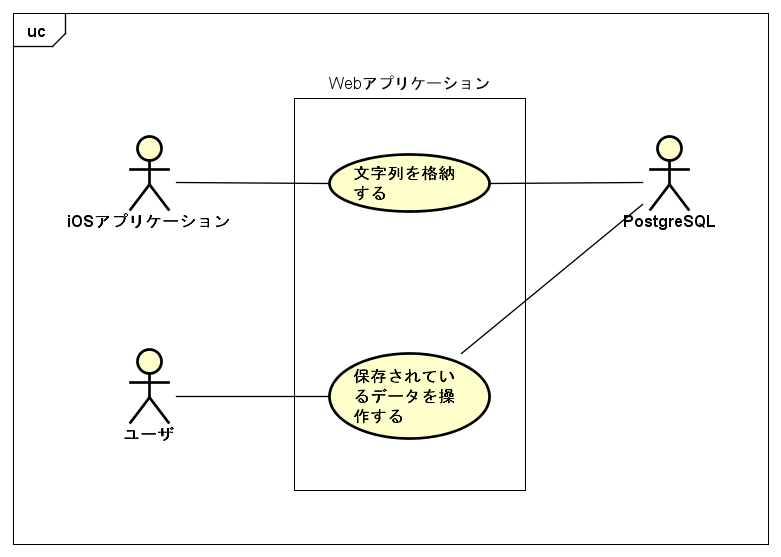
\includegraphics[width=16cm]{fig/usecase_web.png}
\end{center}
\caption{Webアプリケーションのユースケース図}
\end{figure}

\newpage

\subsection{クラス}

\begin{figure}
\begin{center}
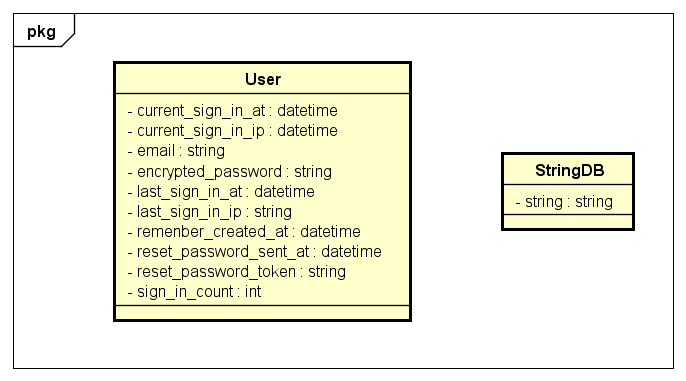
\includegraphics[width=16cm]{fig/class_web.png}
\end{center}
\caption{Webアプリケーションのクラス図}
\end{figure}

\begin{description}

\item (A) Userクラス
\begin{itemize}
\item 属性

\begin{breakbox}
\begin{itemize}
\item current\_sign\_in\_at:datetime

Webアプリケーションにユーザ登録したユーザがサインインした時刻を記録するカラム.

\item current\_sign\_in\_ip:datetime

ユーザがサインインした際のリモートIPを記録するカラム.

\item email:string

ユーザのサインイン時に利用するEメールアドレスを記録するカラム.

\item last\_sign\_in\_at:datetime

ユーザが最終サインインした時刻を記録するカラム.

\item last\_sign\_in\_ip:datetime

ユーザが最終サインインした際のリモートIPを記録するカラム.

\item remenber\_created\_at:datetime

ユーザ登録した時刻を記録するカラム.

\item reset\_password\_sent\_at:datetime

パスワードをリセットする操作を行った際の時刻を記録するカラム.

\item reset\_password\_token:string

パスワードをリセットする操作を行った際に設定した新しいパスワードを記録するカラム.

\item sign\_in\_count:int

ユーザがサインインした回数を記録するカラム.
\end{itemize}
\end{breakbox}

\end{itemize}

\item (B) StringDBクラス
\begin{itemize}
\item 属性

\begin{screen}
\begin{itemize}
\item string:string

光学的文字認識にて取得した文字列を記録するカラム.
\end{itemize}
\end{screen}

\end{itemize}

\end{description}

\section{本システムの評価}
本研究にて構築したシステムは, 「ナンバープレートから取得してきたナンバーの認識の正確性」が大きな要となる.
本節では, Tesseract-OCRのによる光学的文字認識の正確性を評価する.

\subsection{評価方法}
今回は, 「ナンバープレートを撮影することで得られる文字列」と「ナンバープレートを撮影した際に取得することが望ましい文字列」を比較し, ナンバープレートのどの領域で, どの程度の正確な識字を行えているかで, iOSアプリケーションの文字認識の識字率を評価する.

\subsection{評価}
今回, 評価に使用するナンバープレートを撮影した画像(図3.7)を, iOSアプリケーションに内部処理させ, 光学的文字認識を行った結果, 以下のようになった. 

\begin{figure}
\begin{center}
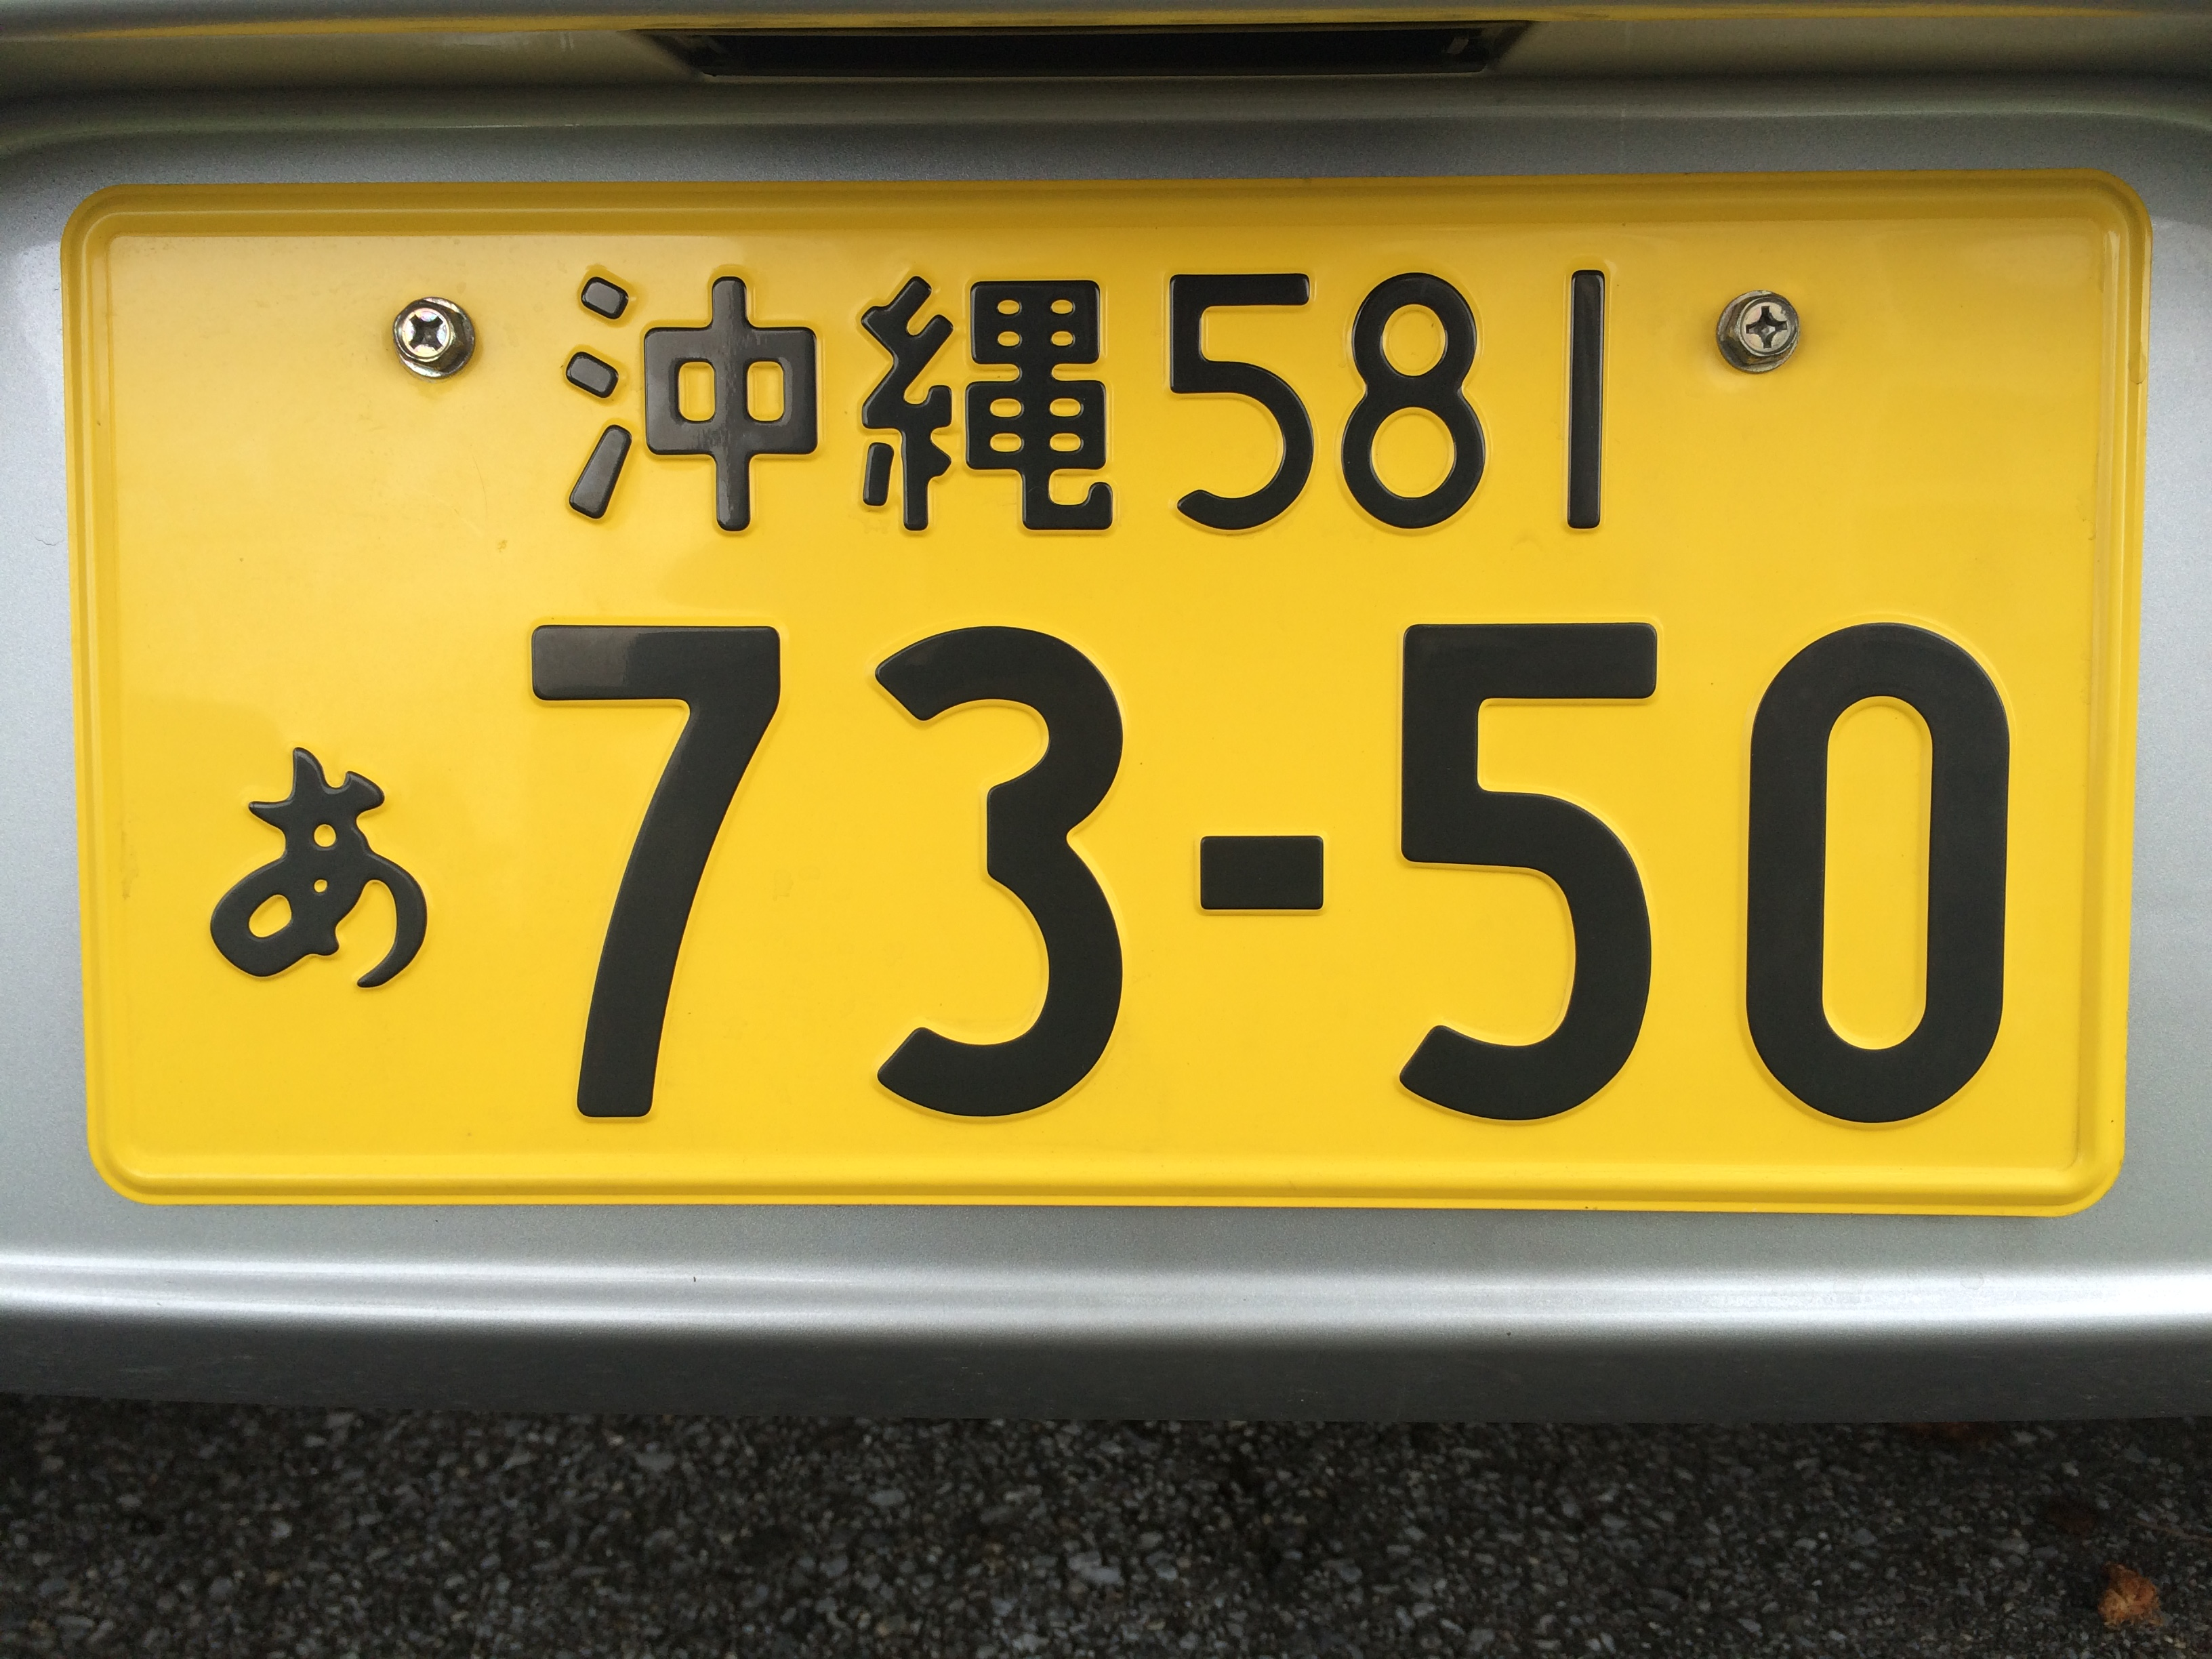
\includegraphics[width=10cm]{fig/IMG_3104.JPG}
\end{center}
\caption{評価に使用した撮影画像}
\end{figure}

\begin{figure}
\begin{center}
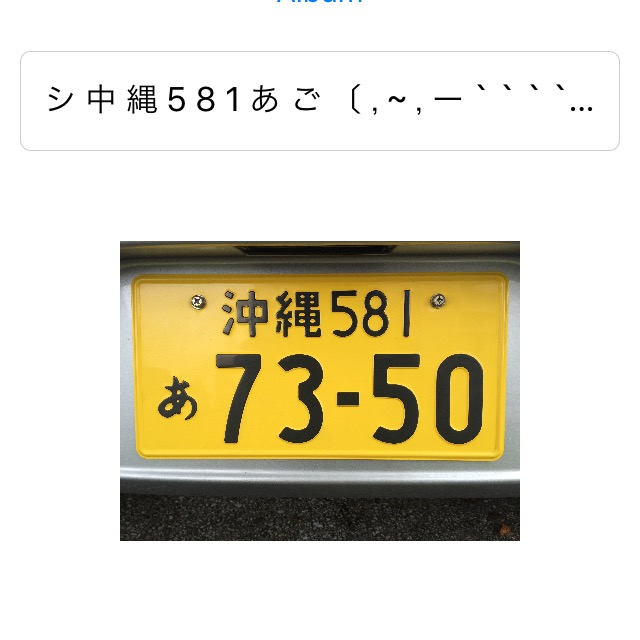
\includegraphics[width=10cm]{fig/FullSizeRender.jpg}
\end{center}
\caption{iOSアプリケーションにて取得したナンバー}
\end{figure}

\begin{itembox}[l]{取得することが望ましい文字列}
「沖縄 581 あ 73-50」
\end{itembox}

\begin{itembox}[l]{実際に取得した文字列}
「シ 中 縄 5 8 1 あ ご 〔 , ~ , ー ` ` ` ` 一 ` 膚 `: ' ` … i ` ` , ` ` 〇 〇 繍 [ y ノ ` ー 〟 ・ 〇 丶 ” ~ ` 〝 / 、 ` 繍〝 閤 ー ` ” V , 退` ` 〝 ' 繍 〝 [ 」 一〟〉~ ー一r'=ヮ'ナノソ~のゲ」
\end{itembox}

取得した文字列と取得したい理想の文字列を比較すると, 「沖縄」, 「581」, 「あ」の部分は文字の形を捉えているが, 「73-50」の部分は全く読み取れていない事が分かる.
文字サイズの小さい 「沖縄」, 「581」, 「あ」の部分が文字として認識されているのに対し, 文字サイズの小さい「73-50」の部分が文字として認識されていないことから, Tesseract-OCRでは, 
\begin{enumerate}
\item バイナリ画像ファイルの黒色領域を認識した際, 領域の大きさで文字列か否かの判定を行う.
\item その黒色領域を文字列で塗りつぶすような処理を施す.
\end{enumerate}
のだと考えられる.

\subsection{問題の解決案}
この問題を解決するためには, 「文字サイズの大きな車両ナンバー部分」が「黒色領域である」と認識されないようにしなければならない.

よって, 以下の処理アルゴリズムを実装することが必要となる.
\begin{itemize}
\item 撮影したナンバープレートを「上部の地域名+数字部分」, 「左端のひらがな部分」, 「4桁のナンバー部分」に分割して注目し, それら領域ごとに光学的文字認識を実行する.
\end{itemize}

文字サイズを基準とした領域ごとに分割して光学的文字認識を施すことで, 文字サイズによる「黒色領域である」という誤判定を発生させず, より正確な文字認識が可能となると考える.

\begin{figure}
\begin{center}
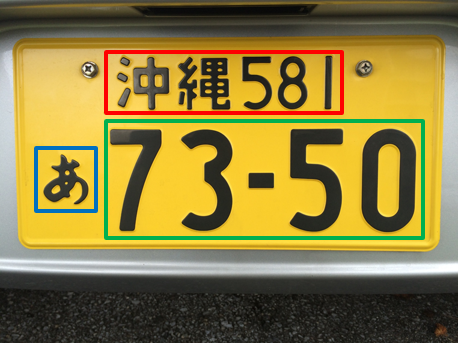
\includegraphics[width=10cm]{fig/hoge.PNG}
\end{center}
\caption{ナンバープレートの文字認識領域の分割例}
\end{figure}
